%
% Created 27 February 2011
%

\chapter[BigBite Magnet]{BigBite Rotation 
\footnote{Author: D. W. Higinbotham \email{doug@jlab.org}}
}

\section{Overview}
The BigBite system is rotated using either a hand operated or an electric wench.
Rotation can only be done locally and needs to be done only after careful inspection that
the nothing will be pulled or damaged by the rotation.  This included not only the cables
attached to BigBite, but also items around BigBite or that may have inadvertently been attached 
to BigBite.  Care most also be taken to move the hundreds of cables that are connected between BigBite
and the DAQ.

\section{Location of Equipment}

All required equipment is located in Hall A.  During operation, the BigBite magnet 
will be located near the pivot area and the BigBox power supply is
located near the Hall A control racks.

\section{Hazard Analysis}

The hazards associated with the rotation of BigBite include:

\noindent{\textbf{Collisions}}
During a rotation, it is possible for BigBite to collide with other items in the Hall.
Along with collisions, items can also be pulled by BigBite.

\noindent{\textbf{DAQ Cables:}}
There are several hundred cables that go between BigBite and the DAQ.  These can easily
be damaged during a BigBite rotation.

\noindent{\textbf{Electrical:}}	The power supply has a maximum output current of 1050~A 
at a voltage of 250~V and thus presents a potentially lethal hazard.  
A hazard also arises from the power bus on the magnet itself. 

\noindent{\textbf{Magnetic:}}	The magnet produces a central field of 0.92~T at 518~A.  
As the magnet has a return yoke and a front field clamp, the external field is much smaller 
than the central field.   Although the magnetic field is primarily confined to the magnet 
gap, fringe fields are strong enough to accelerate unsecured metal objects in the vicinity of
the magnet.  In addition these fields may present a particularly large hazard 
to individuals using a pacemaker.

\section{Hazard Mitigation}

\noindent{\textbf{Collisions}}

To avoid collisions of BigBite with other equipment, careful inspection much be made of the area.
In particular, one needs to out only watch-out for items that BigBite it moving toward, but also check
for items being pulled.  In particular, watch out for items that may have inadvertently been attached to BigBite.
Fig.~\ref{rope-hazard} shows a real world example of a rope having been placed between BigBite and a pipe
and not being found before a rotation.

\begin{figure}[htb]
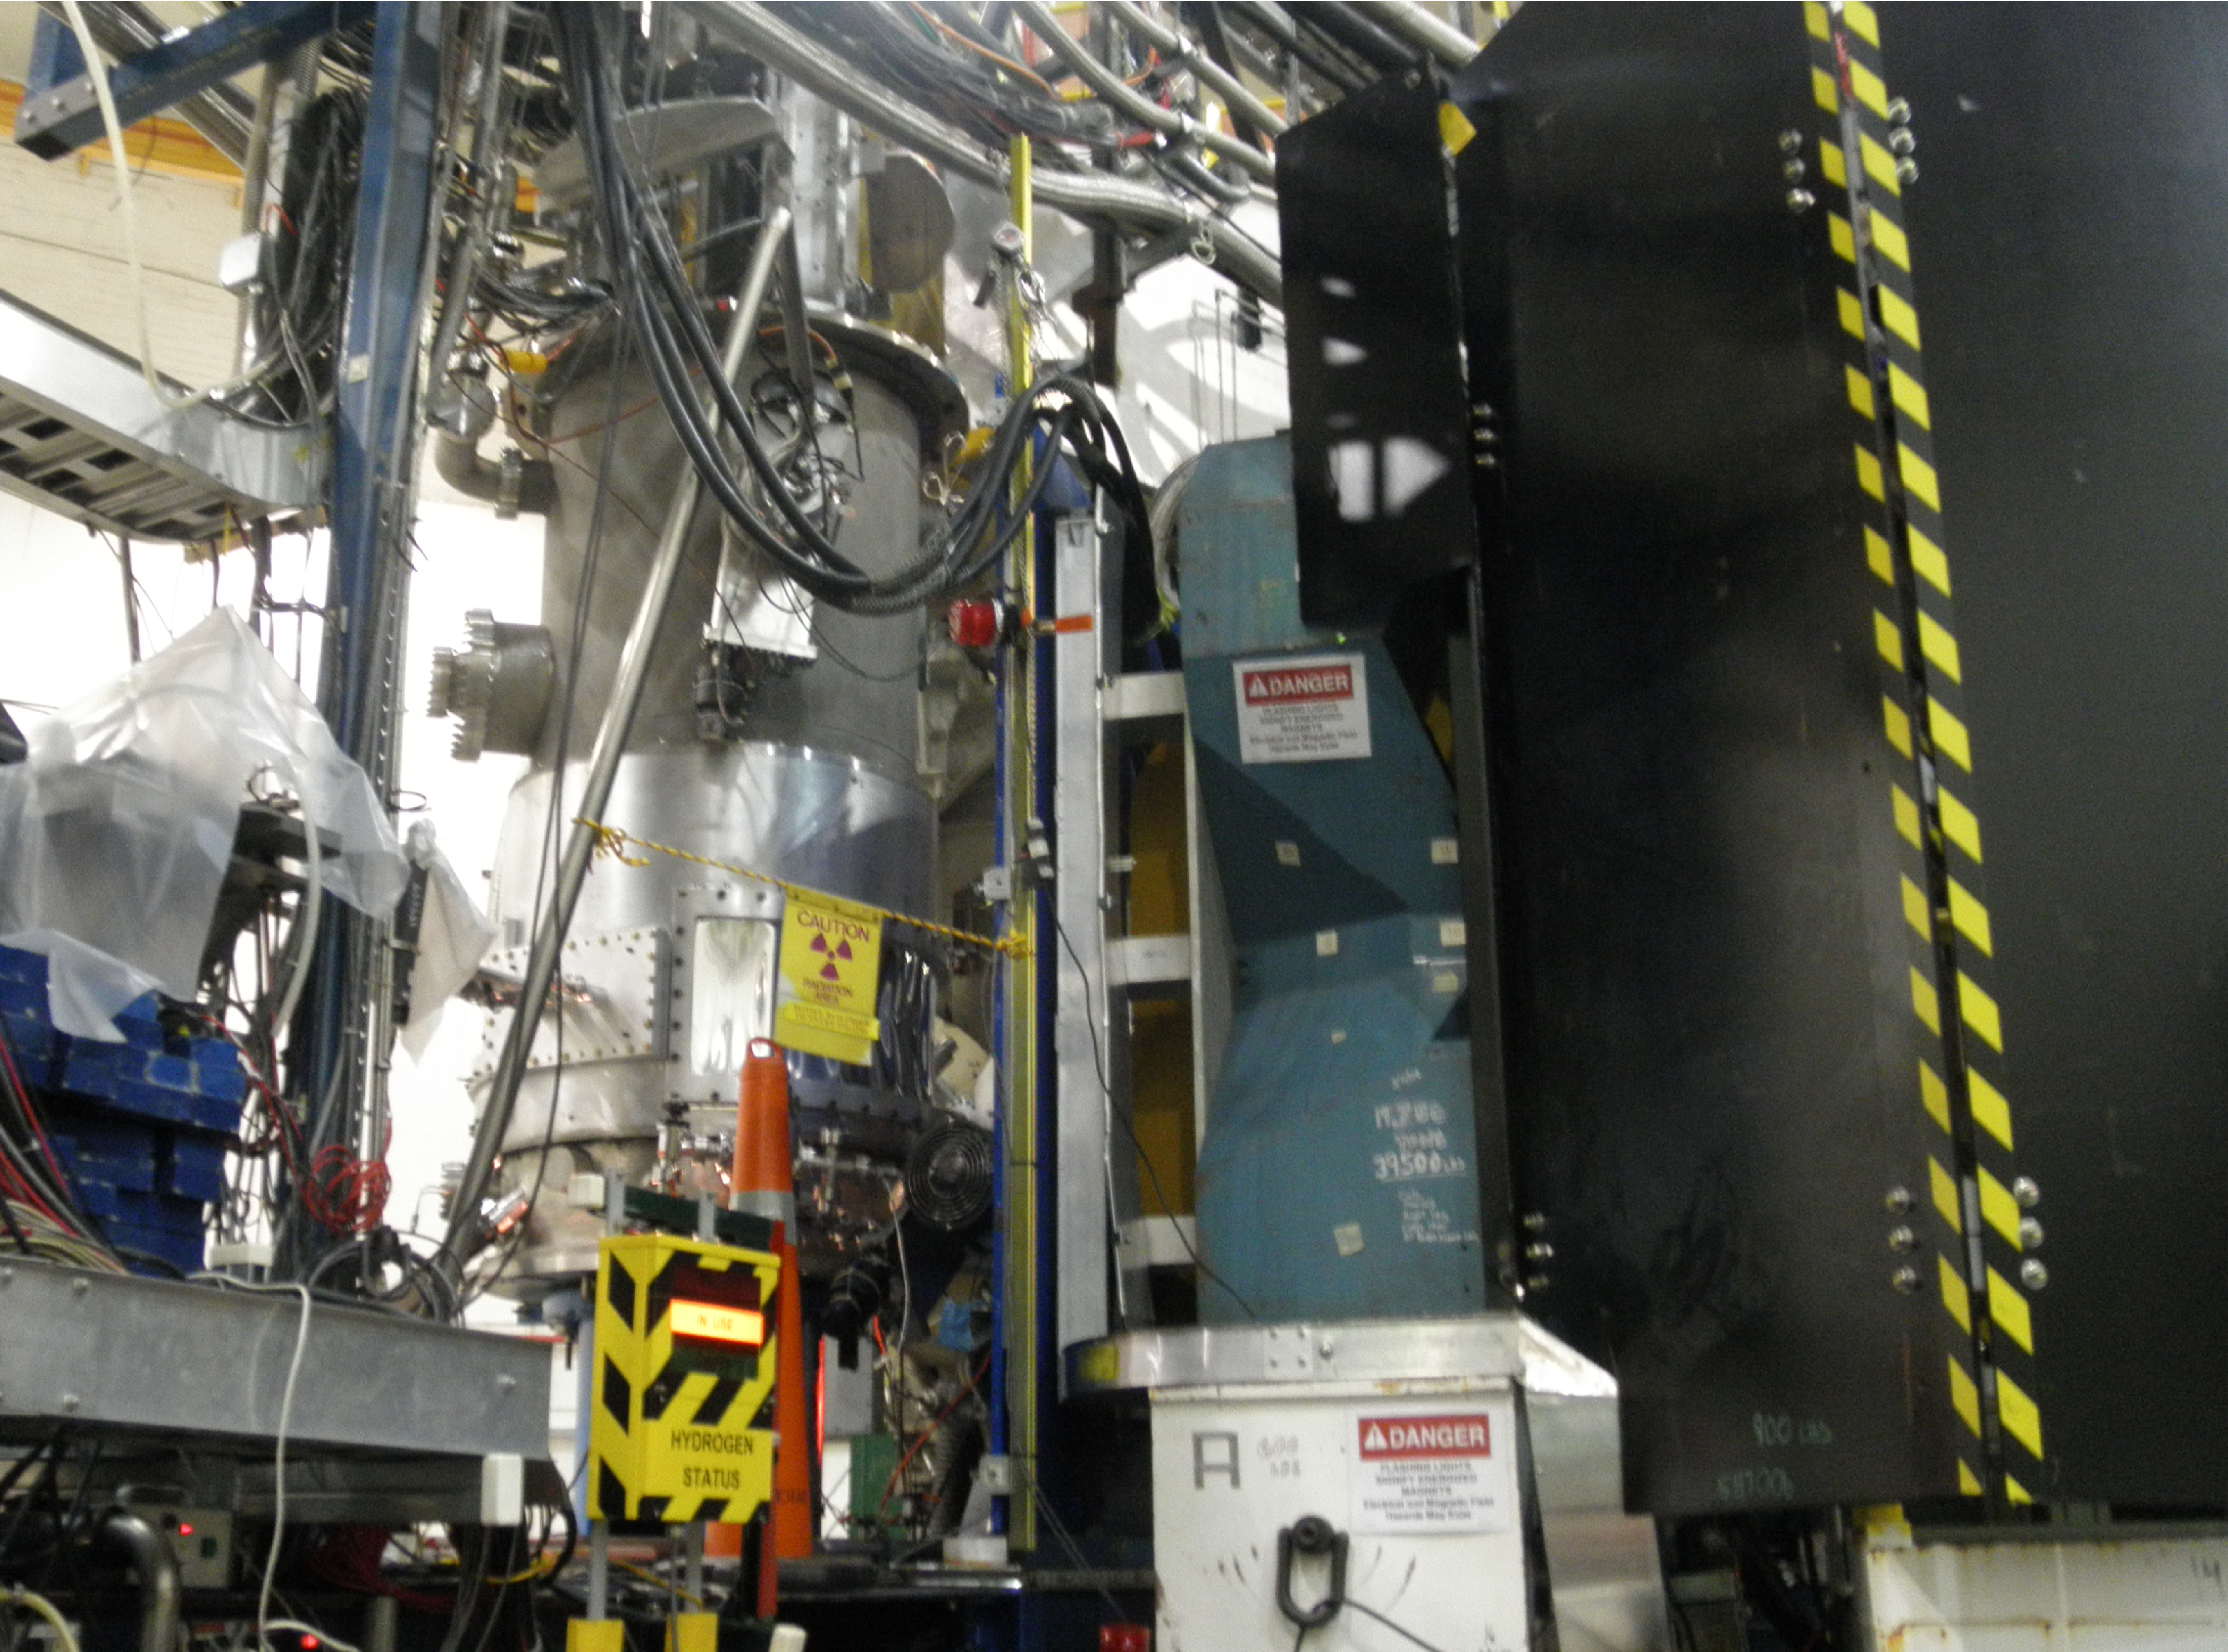
\includegraphics[width=\textwidth]{rope-at-target.pdf}
\caption{Photo of damaged caused by failure to find a rope that had been attached between BigBite
and a pipe.}
\label{rope-hazard}
\end{figure}

\noindent{\textbf{Electrical:}}
The BigBite magnet should be de-energized during rotations and workers should be mindful to watch that
no cables are being damaged by the rotation.  No one should be near the magnet's power bus during
a rotation.

\noindent{\textbf{DAQ Cables:}}
There are several hundred cables that go between BigBite and the DAQ.  These need to be moved along with
BigBite by hand and people need to take care that they are not damaged during the rotation.

\noindent{\textbf{Magnetic:}}
The BigBite magnet should be de-energized during rotations.

\section{Operating Guidelines}

\begin{itemize}
\item{At least two qualified persons must be working on the task together.}
\item{Check area for any potential collisions or attachments.}
\item{One person should be helping to move BigBite cables while the other is operating
the wench.}
\item{Enter record of the rotation into the Hall A electronic log book.}
\end{itemize}

\section{Authority and Responsibility}

The wench may be operated by the Hall A technical staff and people who have been train by the
staff on the use of the wench.  Anyone who has completed the Hall A safety walk-through may act 
as an observer and help move the BigBite cables along.

